

\tikzset{every picture/.style={line width=0.75pt}} %set default line width to 0.75pt        

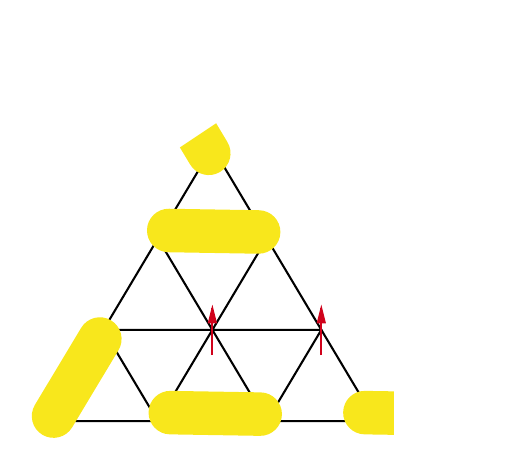
\begin{tikzpicture}[x=0.75pt,y=0.75pt,yscale=-0.75,xscale=0.75]
%uncomment if require: \path (0,300); %set diagram left start at 0, and has height of 300

%Shape: Triangle [id:dp7709012666212918] 
\draw   (292,174.46) -- (327,233.12) -- (257,233.12) -- cycle ;
%Shape: Triangle [id:dp9295040886868511] 
\draw   (222,174.46) -- (257,233.12) -- (187,233.12) -- cycle ;
%Shape: Triangle [id:dp177949788580418] 
\draw   (257,115.79) -- (292,174.46) -- (222,174.46) -- cycle ;
%Shape: Triangle [id:dp03247866415223255] 
\draw   (362,174.46) -- (397,233.12) -- (327,233.12) -- cycle ;
%Shape: Triangle [id:dp26037578632796765] 
\draw   (327,115.79) -- (362,174.46) -- (292,174.46) -- cycle ;
%Shape: Triangle [id:dp3012062348071127] 
\draw   (292,57.12) -- (327,115.79) -- (257,115.79) -- cycle ;
%Rounded Rect [id:dp4030558357818268] 
\draw  [draw opacity=0][fill={rgb, 255:red, 248; green, 231; blue, 28 }  ,fill opacity=1 ] (182.79,241.83) .. controls (176.17,237.86) and (174.03,229.28) .. (178,222.66) -- (207.75,173.14) .. controls (211.72,166.53) and (220.3,164.39) .. (226.92,168.36) -- (226.92,168.36) .. controls (233.53,172.33) and (235.67,180.92) .. (231.7,187.53) -- (201.96,237.05) .. controls (197.99,243.66) and (189.4,245.81) .. (182.79,241.83) -- cycle ;
%Rounded Rect [id:dp16737425370308645] 
\draw  [draw opacity=0][fill={rgb, 255:red, 248; green, 231; blue, 28 }  ,fill opacity=1 ] (250.01,110.39) .. controls (250.13,102.67) and (256.49,96.52) .. (264.21,96.65) -- (321.96,97.61) .. controls (329.68,97.73) and (335.83,104.09) .. (335.7,111.81) -- (335.7,111.81) .. controls (335.57,119.52) and (329.21,125.67) .. (321.5,125.55) -- (263.74,124.59) .. controls (256.03,124.46) and (249.88,118.1) .. (250.01,110.39) -- cycle ;
%Rounded Rect [id:dp7997977143532831] 
\draw  [draw opacity=0][fill={rgb, 255:red, 248; green, 231; blue, 28 }  ,fill opacity=1 ] (251.01,227.39) .. controls (251.13,219.67) and (257.49,213.52) .. (265.21,213.65) -- (322.96,214.61) .. controls (330.68,214.73) and (336.83,221.09) .. (336.7,228.81) -- (336.7,228.81) .. controls (336.57,236.52) and (330.21,242.67) .. (322.5,242.55) -- (264.74,241.59) .. controls (257.03,241.46) and (250.88,235.1) .. (251.01,227.39) -- cycle ;
%Straight Lines [id:da8204619655647556] 
\draw [color={rgb, 255:red, 208; green, 2; blue, 27 }  ,draw opacity=1 ]   (292,190.68) -- (292,160.23) ;
\draw [shift={(292,158.23)}, rotate = 450] [fill={rgb, 255:red, 208; green, 2; blue, 27 }  ,fill opacity=1 ][line width=0.08]  [draw opacity=0] (12,-3) -- (0,0) -- (12,3) -- cycle    ;
%Straight Lines [id:da301443667677862] 
\draw [color={rgb, 255:red, 208; green, 2; blue, 27 }  ,draw opacity=1 ]   (362,190.68) -- (362,160.23) ;
\draw [shift={(362,158.23)}, rotate = 450] [fill={rgb, 255:red, 208; green, 2; blue, 27 }  ,fill opacity=1 ][line width=0.08]  [draw opacity=0] (12,-3) -- (0,0) -- (12,3) -- cycle    ;
%Rounded Rect [id:dp28390331250432066] 
\draw  [draw opacity=0][fill={rgb, 255:red, 248; green, 231; blue, 28 }  ,fill opacity=1 ] (376.01,227.39) .. controls (376.13,219.67) and (382.49,213.52) .. (390.21,213.65) -- (447.96,214.61) .. controls (455.68,214.73) and (461.83,221.09) .. (461.7,228.81) -- (461.7,228.81) .. controls (461.57,236.52) and (455.21,242.67) .. (447.5,242.55) -- (389.74,241.59) .. controls (382.03,241.46) and (375.88,235.1) .. (376.01,227.39) -- cycle ;
%Shape: Rectangle [id:dp4527570591753749] 
\draw  [draw opacity=0][fill={rgb, 255:red, 255; green, 255; blue, 255 }  ,fill opacity=1 ] (409,207) -- (473.71,207) -- (473.71,247) -- (409,247) -- cycle ;
%Rounded Rect [id:dp3963770711962662] 
\draw  [draw opacity=0][fill={rgb, 255:red, 248; green, 231; blue, 28 }  ,fill opacity=1 ] (252.81,-0.47) .. controls (259.43,-4.44) and (268.01,-2.29) .. (271.98,4.32) -- (301.69,53.86) .. controls (305.66,60.48) and (303.51,69.06) .. (296.89,73.03) -- (296.89,73.03) .. controls (290.27,77) and (281.69,74.85) .. (277.72,68.23) -- (248.02,18.69) .. controls (244.05,12.08) and (246.2,3.49) .. (252.81,-0.47) -- cycle ;
%Shape: Rectangle [id:dp5531026767203489] 
\draw  [draw opacity=0][fill={rgb, 255:red, 255; green, 255; blue, 255 }  ,fill opacity=1 ] (264.79,61.43) -- (225.94,3.2) -- (259.21,-19) -- (298.06,39.23) -- cycle ;




\end{tikzpicture}
